\chapter{ВЫБОР ФИЗИЧЕСКИХ ПАРАМЕТРОВ СКАНЕРА}
    В результате обзора аналогов стало ясно, что использовать готовые решения для нашей системы невозможно. Таким образом необходимо разработать собственный модуль совместимый с прототипом. Для этого требуется с учётом особенностей принтера выбрать подходящий метод сканирования, компоновку модуля и составляющие модуля.
    \section{Выбор метода сканирования}
        Для выбора метода сканирования необходимо выделить условия работы и ограничения накладываемые существующей конструкцией на модуль и сопоставить их с требованиями и особенностями методов, а также учесть требования технического задания.
        
        Поскольку все методы оптические, они предъявляют требования к освещению окружения. Оно не должно быть неравномерным, не должно быть слишком ярким и должно быть без бликов. При этом сканируемые поверхности не должны быть зеркальными или поглощающими свет.
        
        Параметры конструкции принтера:
        \begin{itemize}
            \item габариты принтера $ 400 \times 550 \times 560 \text{ мм} $
            \item размеры стола $ 200 \times 200 \text{ мм} $
            \item контролируемое освещение
            \item закрытый корпус
        \end{itemize}
        
        Видно, что свободное пространство в принтере ограничено, особенно учитывая наличие подвижного печатающего узла, габариты которого выходят за пределы рабочей зоны. Таким образом становится невозможно использование крупных компонентов в нашем модуле, даже если они стационарные.

        Поэтому метод структурированного света в данном случае не подходит, так как требует использование проектора, которые имеют большие размеры и не дёшевы. Существуют и миниатюрные проекторы, однако их цены ещё выше. Помимо этого алгоритмы для расчёта координат по этому методу довольно сложны.

        Лазерная триангуляция накладывает дополнительные ограничения на возможные сканируемые поверхности, так как использует видимое излучение для работы. Это значит, что сканирование в свете предметов такого-же цвета, что и свет излучаемый лазером, будет сильно затруднено. Такая ситуация может возникнуть, если изделие, например торт, будет обладать цветным покрытием. Однако это можно преодолеть если использовать сканирование в темноте. Это позволит сканировать такие объекты, тем не менее качество таких сканов будет хуже из-за явления самозасветки лазера.
        Так же, используя этот метод, модуль, целиком или только лазер, необходимо перемещать вдоль сцены, чтобы захватить все профили исследуемой поверхности. Это снизит скорость сканирования в сравнении с остальными методами.
        Однако для реализации этого метода достаточно одной камеры и лазерного модуля. Это позволяет компактно расположить элементы, так как они не занимают много места. Так же это позволяет не тратить больших средств, что важно в данном проекте.

        Метод фотограмметрии или стереозрения в данной работе не рассматривается, так как этот метод был опробован ранее и не показал удовлетворительных результатов. В данном методе теряется большое количество данных сцены и точность оставляет желать лучшего. При этом для этого необходимы две камеры, что так же проблематично встроить в существующую систему\cite{SkripkoPASEKA}.
        
    \section{Выбор компоновки}
        Общий план модуля сканирования представлен на рисунке \ref{pic:general_view} (подвижный узел не показан). Он демонстрирует относительное расположение элементов в пространстве. В данной компоновке лазер направлен перпендикулярно столу (параллельно оси $ Z $), линия проекции параллельна оси $ Y $ стола, а камера под углом к вертикали -- вокруг оси $ Y $ системы координат стола -- не имея поворота относительно остальных осей. При этом из-за особенностей конструкции камера получается расположена <<вверх-ногами>>. Движение модуля происходит параллельно оси $ X $ системы координат принтера в сторону уменьшения координаты.

        \cbox{убрать подпись в углу картинки}

        \begin{figure}[H]
            \centering
            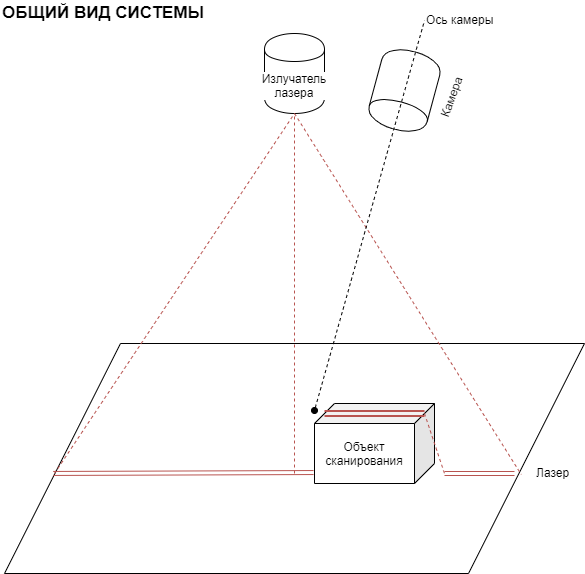
\includegraphics[width=0.5\linewidth]{general_view}
            \caption{Общий план модуля}
            \label{pic:general_view}
        \end{figure}

        Для обеспечения лучших показателей точности необходимо выбрать расстояние и угол между оптической осью камеры и осью лазера, а так же расстояние от камеры до стола. Этот этап важен, так как от этих параметров зависит разрешающая способность сканера и видимая рабочая зона. Чем ниже камера к столу, тем меньше дискретизация значений координат, но одновременно меньше видимая область. Угол наклона камеры также влияет на дискретизацию и видимую область сканера.
        С помощью расчётов приведённых в разделе \ref{sec:error} были установлены следующие величины этих размеров:
        \begin{table}[H]
            \centering
            \caption{Основные размеры модуля сканирования}\label{table:dims}
            \begin{tabular}{|l|c|} \hline
                Высота над столом& $ 150  \pm 10 \text{ мм} $\\ \hline
                Расстояние от камеры до лазера& $ 150  \pm 10 \text{ мм} $\\ \hline
                Угол между осями камеры и лазера& $ 30-45\degs $\\ \hline
            \end{tabular}
        \end{table}
        Данные величины позволяют достичь необходимой по ТЗ точности в $ \pm 0.5 \text{ мм} $ и ширины обзора 200 мм.
        Для модуля используется камера Microsoft Lifecam Cinema с максимальным разрешением $ 1080 
        \times 720 $ и максимальной частотой 30 кадров в секунду. Использование данной камеры позволяет упростить процесс калибровки, так как она обладает встроенной ректификацией изображения. Лазерный модуль S-2S с толщиной проецируемой линии в 3 мм. Толщина линии лазера также влияет на точность измерений и в общем случае чем тоньше, тем лучше.

        Камера устанавливается в специальный держатель изготовленный по технологии 3D-печати, в котором предусмотрена калибровка поворота камеры для более точного направления на интересующую зону и надёжного закрепления. Реализация крепления и установки модуля в систему рассматривается в работе\cite{matsu}. 

        К конструкции модуля предъявляются следующие требования:
        \begin{itemize}
            \item минимизация влияния вибрации на положение камеры
            \item размеры в пределах указанных в таблице \ref{table:dims}
            \item минимизация видимой части препятствий
            \item допускаются препятствия в верхней половине кадра занимающие не более четверти высоты кадра
            \item возможность калибровки поворота камеры
            \item возможность калибровки поворота лазера
        \end{itemize}
    
        Итоговый вид модуля в составе системы изображён на рисунке \ref{pic:final_model}. Крепление камеры изображена на рисунке \ref{pic:camera_mount}.

        \begin{figure}[H]
            \centering
            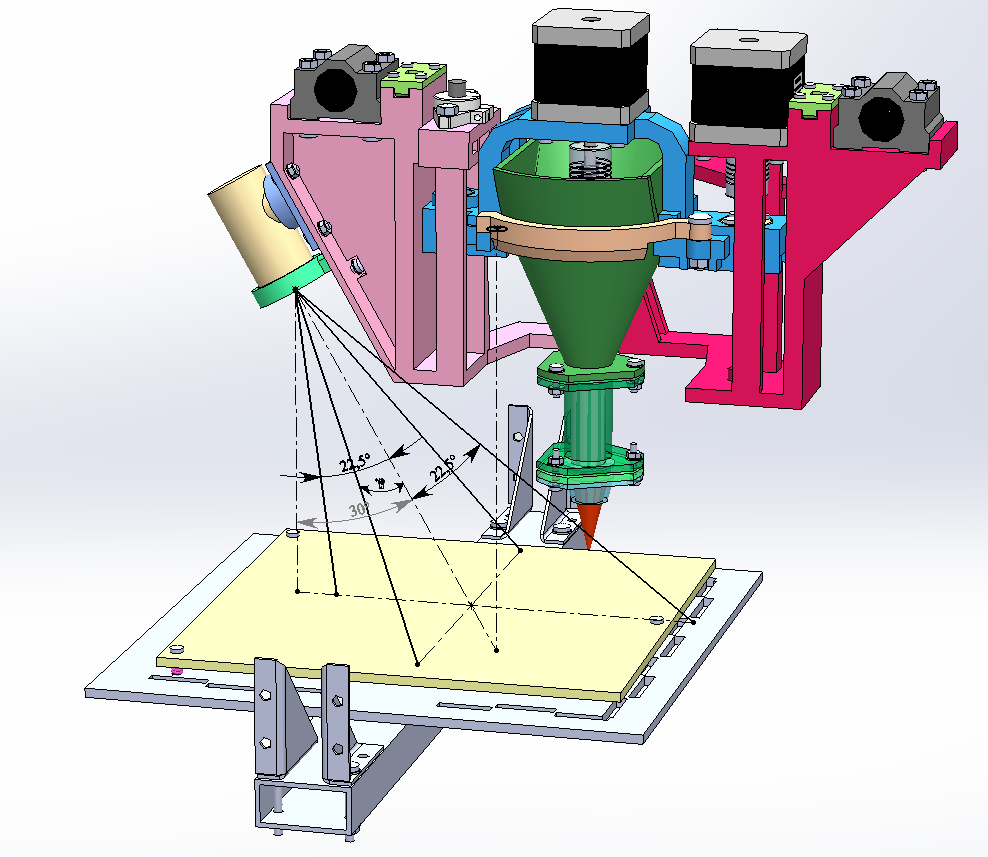
\includegraphics[width=\linewidth]{final_model_camera_view}
            \caption{Общий вид в принтере}
            \label{pic:final_model_camera_view}
            \cbox{СДЕЛАТЬ НОРМ СКРИН}
        \end{figure}
        
        \begin{figure}[H]
            \centering
            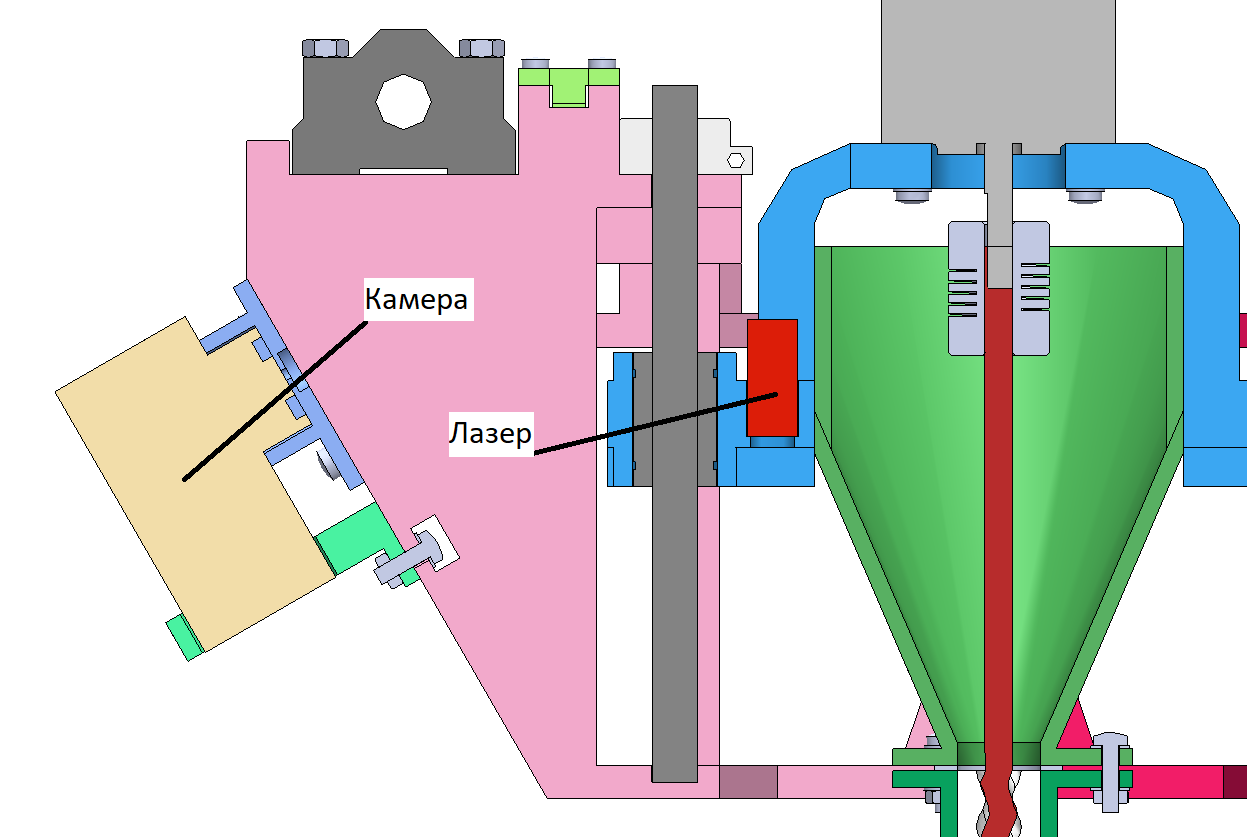
\includegraphics[width=\linewidth]{final_model_capts}
            \caption{Финальная компоновка модуля сканирования}
            \label{pic:final_model}
        \end{figure}
    
        \begin{figure}[H]
            \centering
            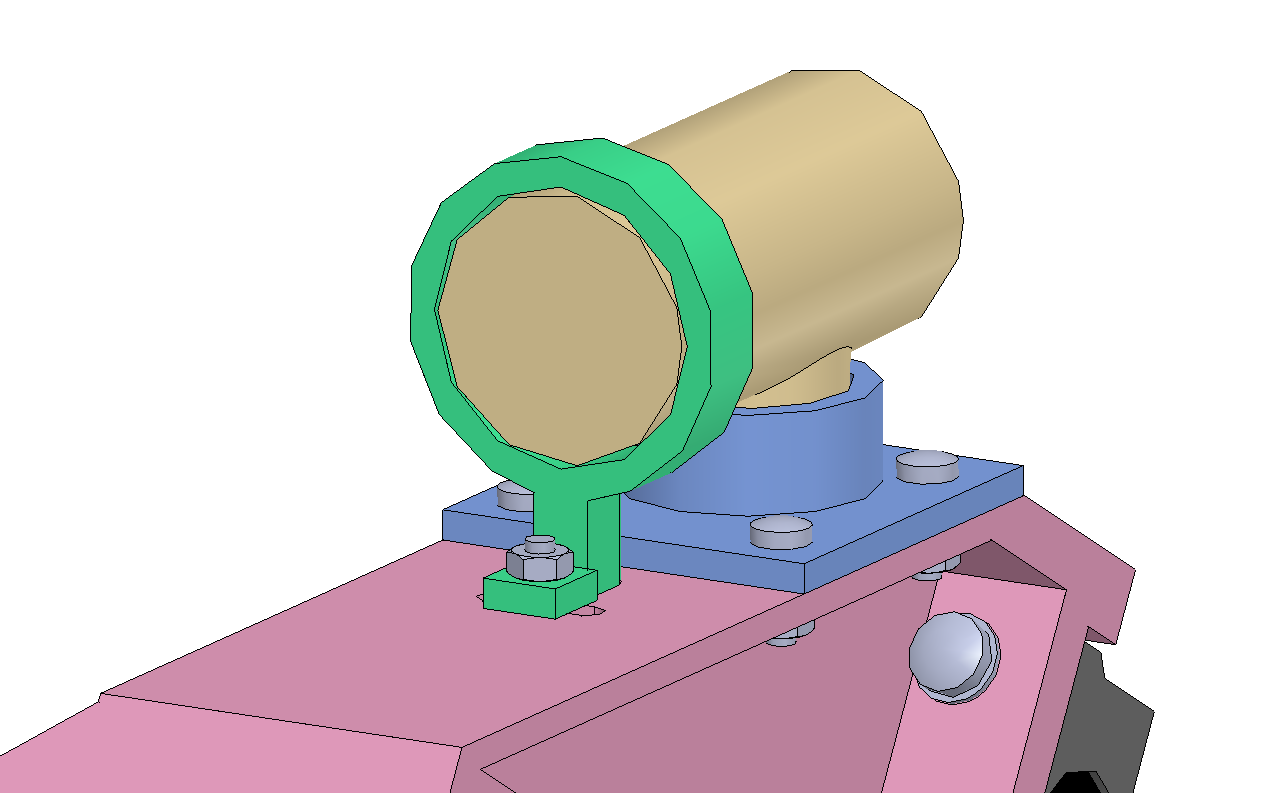
\includegraphics[width=0.5\linewidth]{camera_mount}
            \caption{Крепление камеры}
            \label{pic:camera_mount}
        \end{figure}